\documentclass[a4paper,11.5pt,table]{article}
\usepackage[textwidth=170mm, textheight=230mm, inner=20mm, top=20mm, bottom=30mm]{geometry}
\usepackage[normalem]{ulem}
\usepackage[utf8]{inputenc}
\usepackage[T1]{fontenc}
\PassOptionsToPackage{defaults=hu-min}{magyar.ldf}
\usepackage[magyar]{babel}
\usepackage{amsmath, amsthm, amssymb, paralist, tikz, multirow}
\usetikzlibrary{arrows, positioning}

\usepackage{listings}
\lstset{
	language=C++, 
	basicstyle=\ttfamily, 
	keywordstyle=\color{blue}\ttfamily, 
	stringstyle=\color{red}\ttfamily,
	tabsize = 4
}

\usepackage{hyperref}

\begin{document}
	%%%%%%%%%%%RÖVIDÍTÉSEK%%%%%%%%%%
	\setlength\parindent{0pt}
	\def\<{<\hspace{0mm}<}
	
	\theoremstyle{definition}
	\newtheorem{note}{Megjegyzés}[subsection]
  \newtheorem{example}{Példa}[subsection]
  \newtheorem{definition}{Definíció}[subsection]
	%%%%%%%%%%%%%%%%%%%%%%%%%%%%%%%%%%%%%%%%%%%%%%%%%%%%%%%%%%%%%%%%%%%%%

	
	\begin{center}
		{\LARGE\textbf{C++}}
		
		{\Large Gyakorlat jegyzet}
		
		3 óra.
	\end{center}
	A jegyzetet \textsc{Umann} Kristóf készítette \textsc{Porkoláb} Zoltán és \textsc{Horváth} Gábor gyakorlata alapján. (\today)
%	\section{Kifejezések kiértékelése}
%	Ugorjunk vissza egy korábbi példára.
%	\begin{lstlisting}
%#include <iostream>
%
%int main()
%{
%	int i = 0;
%	std::cout << i << i++ << std::endl;
%}
%	\end{lstlisting}
%	%\< egy normálisabban kinéző << operátort eredményez (definíció fent)
%	
%	Világos, hogy a fenti kódban nem definiált viselkedés szerepel. Már volt szó arról is, hogy a kiíratáshoz használt \texttt{\<} szimbólum az egy operátor, és az \texttt{<iostream>} könyvtárban található hozzá egy olyan overload, melynek egyik paramétere \texttt{std::ostream\&}, a másik pedig \texttt{int}. Ahogy korábban is említettük, az első paramétert adja vissza, így tudjuk a kiíratást láncolni. A fent leírt kiíratás ezzel lesz ekvivalens:
%	\begin{lstlisting}
%std::cout.operator<<(i).operator<<(i++);
%	\end{lstlisting}
%	
%	Itt látható egy \texttt{\<} operátor, ami így is felírható: \texttt{std::cout.operator$<<$(i)}. Ennek a függvényhívásnak van visszatérési értéke, méghozzá \texttt{std::cout}, ez teszi lehetővé a láncolást. Ez itt egy tagfüggvény, mely majdnem minden alaptípusra túl van terhelve. 
%	
%	Az biztos, hogy a második kiírt szám értéke 2. De az, hogy az első mennyi, nem definiált.
%	
%	\begin{example}
%		\texttt{x = k + 2}\quad \quad \texttt{y = k + 2}
%	\end{example}
%	
%	Ebben a példában (jó eséllyel) a fordító optimalizál, és \texttt{k+2}-t csak egyszer számolja ki. A C++ban szabvány által nem definiált viselkedéseknek köszönhetően sokkal hatékonyabb programokat kaphatunk, mert a fordítónak nagy szabadsága van abban, hogyan optimalizáljon.
%	
%	\begin{example}
%		Töltsük fel egy tömb elemeit növekvő sorrendben számokkal.
%		
%		\begin{lstlisting}
%int i = 0;
%int t[10];
%while (i < 10)
%{
%	t[i] = i++;
%}
%		\end{lstlisting}
%		
%		A kód viselkedése ismét nem definiált. Hiába van ott egy \textbf{post-fix} \texttt{++}\quad operator. Az, hogy az értékadás melyik oldalán levő \texttt{i} értékelődik ki először, nem specifikált.
%	\end{example}
%	
%	A szekvenciapontok korrekt használatával lehet kijavítani a fenti kódot.
%	
%	\begin{definition}
%		(Szekvenciapont) meghatározza a kifejezések kiértékelési sorrendjét futási időben. A szekvenciapont előtti kifejezéseknek hamarabb ki kell értékelődnie, mint a szekvenciapont utániaknak. Néhány példa szekvenciapontokra: vessző, \texttt{\&\&}, \texttt{||}, \texttt{?\quad :} 
%	\end{definition}
%	\begin{example}
%		\begin{lstlisting}
%f(i), ++i;
%i++<10 && f(i);
%i++<10 || f(i);
%i++<10 ? f(i) : g(i);
%		\end{lstlisting}
%		A fenti példák eredményei mind jól definiáltak, a szekvenciapontok miatt egyértelmű a kifejezések eredménye.
%		\begin{lstlisting}
%f(i++, j++);
%		\end{lstlisting}
%		Itt azonban az, hogy i vagy j értéke növekszik-e meg először, az nem specifikált. Bár valóban található ott vessző, de a vessző operátor mint szekvenciapont nem ekvivalens a függvény paramétereit elválasztó vesszővel.
%	\end{example}
%	
%	\begin{lstlisting}
%int f() {cout << 'f'; return 2;}
%int g() {cout << 'g'; return 1;}
%int h() {cout << 'h'; return 0;}
%	\end{lstlisting}
%	Mi fog történni \texttt{f() == g() == h()} kód írásakor?
%	
%	Itt a kimenet attól is függ, hogy milyen sorrendben értékelődnek ki az egyenlőség-vizsgáló operátorok. Az operátoroknak van megadott precedenciájuk, ami meghatározza mennyire erősen kötnek: erős például a pont, nyíl, [], gyengébb ennél a dereferencia, és így tovább. Azonban az azonos precedenciájú operátoroknál kérdéses, hogy a részkifejezések milyen sorrendben értékelődnek ki. 
%	
%	Visszatérve a fenti példára, a végrehajtási sorrend:
%	\texttt{(f() == g()) == h()}. Azaz, a \texttt{==} operátor balról jobbra zárójelezendő, tehát balasszociatív. Milyen sorrendben lesznek kiírva a karakterek? Ez nem specifikált, hiszen a függvényhívásokat nem választja el egymástól szekvenciapont.
%	
%	Van ahol más a zárójelezés, pl. \texttt{!++*++p}. Itt Először előrelépünk a p pointerrel, dereferáljuk, megnöveljük az értékét, és negáljuk. \texttt{!(++(*(++p)))}. Ilyen példa szintén az egyenlőség operátor: \texttt{x = y = z = 3.14}. 
%	\begin{note}
%		Bővebben: \url{http://en.cppreference.com/w/cpp/language/operator_precedence}
%	\end{note}
%	\begin{lstlisting}
%#include <iostream>
%
%const char* answer (const char *q);
%
%int main()
%{
%	std::cout << answer("Hogy vagy?") << answer("Biztos?") << std::endl;
%	return 0;
%}
%
%const char* answer (const char *q)
%{
%	std::cout << q;
%	static char buffer[80];
%	std::cin.getline(buffer,80);
%	return buffer;
%}
%	\end{lstlisting}
%	A fenti kódban előfordulhat, hogy a két üzenet kiírásának a sorrendje nem megfelelő. 
%	
%	A pontosvessző szekvenciapont, így a megoldás egyszerű:
%	
%	\texttt{std::cout $<<$ answer("Hogy vagy?");}
%	
%	\texttt{std::cout $<<$ answer("Biztos?");}
%	
%	A fenti kódban nem szép, hogy van egy statikus változó a függvényen belül. Azért statikus, hogy a buffer ne szűnjön meg a függvényből való visszatérés után, hiszen abban van a válasz. Egy statikus változó viszont életben van a program befejezéséig, ráadásul az esetleges párhuzamosítást is megakadályozza a későbbiekben.
%	\medskip
%	
%	A dinamikusan lefoglalt memória kezelése a stacken lévő objektumokkal szemben a programozó felelőssége. Nekünk kell lefoglalni, és ha nincs már rá szükségünk, nekünk is kell felszabadítani. C++11ben smart-pointerekkel ezt valamelyest automatizálhatjuk.
%	
%	\begin{lstlisting}
%#include <iostream>
%
%const char* answer (const char *q);
%
%int main()
%{
%	std::cout << answer("Hogy vagy?");
%	std::cout << answer("Biztos?");
%	return 0;
%}
%
%const char* answer (const char *q)
%{
%	std::cout << q;
%	char* buffer = new char[80];
%	std::cin.getline(buffer,80);
%	return buffer;
%}
%	\end{lstlisting}
%	A fenti kódban sajnos a lefoglalt memória elszivárgott. A \texttt{new} kulcsszóval létrehoztunk a dinamikus tárhelyen egy új változót, de azt soha nem szabadítottuk fel. Egy lehetőség lenne az, hogy referencia szerint átadunk egy buffert, amiben el tudjuk tárolni a választ. Annak azonban kényelmetlen a használata. Ennél szebb megoldás, ha az \texttt{std::string}-et használjuk.
%	\begin{lstlisting}
%#include <iostream>
%#include <string>
%
%std::string answer (std::string q);
%
%int main()
%{
%	std::cout << answer("Hogy vagy?");
%	std::cout << answer("Biztos?");
%	return 0;
%}
%
%std::string answer (std::string q)
%{
%	std::cout << q;
%	std::string buffer;
%	std::cin >> buffer;
%	return buffer;
%}
%	\end{lstlisting}
%	
%	Ez a memóriában úgy néz ki, hogy a stacken létrejön egy pointer ami egy heapen foglalt bufferre mutat. Az objektum másolásakor a heapen lévő buffer is másolásra kerül, az objektum megsemmisülésekor a heapen lévő buffer felszabadul. A másolások költségesek lehetnek, azonban a fordító optmializációi és a C++11-es move szemantika sokat javít a hatékonyságon.
%	
	\section{Pointer aritmetika}
	\subsection{Konstans korrektség}
	Térjünk vissza a mutatókhoz. Volt már szó konstans mutatókról, ám konstans\textbf{ra} mutató mutatókról még nem.
	\begin{lstlisting}
const int ci = 6;
int *p = &ci;
	\end{lstlisting}
	A fenti kód nem fordul le, mert \texttt{ci} konstans, de \texttt{p} nem egy nem konstansra mutató pointer. Ez sértené a C++ban ismert \textbf{konstans korrektséget} (const correctness). A probléma forrása az, ha fenti értékadás lefordulna, akkor \texttt{ci} értékét tudnánk módosítani \texttt{p}-n keresztül.
	
	\medskip
	\textbf{Konstans korrektség:} ha egy értéket konstansnak jelölünk, azt nem módosíthatjuk a program futása során. 
	\begin{lstlisting}
const int ci = 6;
const int *p = &ci;
	\end{lstlisting}
	Ez már lefordul, hiszen a \texttt{p} egy konstansra mutató pointer, azaz mutathat konstans változókra. Egy konstansra mutató pointer \textbf{nem tudja megváltoztatni} a mutatott értéket. Viszont egy konstansra mutató mutatót át lehet állítani egy másik memóriacímre.
	\begin{lstlisting}
const int ci = 6;
const int *p = &ci;

int c = 5;
p = &c;
	\end{lstlisting}
	A fenti kód is szabályos, konstansra mutató pointerrel nem konstans is értékre mutathatunk. Érdemes átgondolni ennek a következményeit, hisz \texttt{c} nem konstans, ezért az értékét továbbra is módosíthatjuk (csak nem \texttt{p}-n keresztül)! Egy konstansra mutató mutató nem azt jelenti, hogy a mutatott érték sosem változhat meg. Csupán annyit jelent, hogy a mutatott értéket ezen a mutatón keresztül nem lehet megváltoztatni.
	\begin{lstlisting}
const int *p = &ci;
int c = 5;
p = &c;
c = 5;
	\end{lstlisting}
  A \texttt{const} kulcsszó több helyre is kerülhet.
	\begin{lstlisting}
const int *p;
int const *p;
	\end{lstlisting}
	A fenti két sor ugyanazt jelenti, a mutatott értéket nem lehet megváltoztatni a mutatón keresztül.
	\begin{lstlisting}
int * const p;
const int * const p;
int const * const p;
	\end{lstlisting} 
	Amennyiben a * után van a \texttt{const}, akkor egy \textbf{konstans pointert kapunk}, mely megváltoztathatja a mutatott értéket, de nem mutathat másra (konstans pointer \quad $\not=$\quad konstanra mutató pointer). Egy létezik konstansra mutató konstans mutató is, amin keresztül nem lehet megváltoztatni a mutatott értéket és a mutatót sem lehet máshova átállítani.
	\subsection{Mutatóra mutató mutatók} 
	Mutatóra mutató mutatók is léteznek. Néhány példa:
	\begin{lstlisting}
int *p;
int **q = &p;
int ***r = &q;
	\end{lstlisting}
	Példaképp \texttt{q}-n keresztül meg tudjuk változni, \texttt{p} hova mutasson.
	\begin{lstlisting}
int c, d;
int *p = &c;
int **q = &p;
*q = &d;
	\end{lstlisting}
	A megfelelő szinten a mutatók konstansá tételével még bonyolultabb példákat kaphatunk:
	\begin{lstlisting}
int c, d;
int *p = &c;
int * const *q = &p;
*q = &d; // forditasi hiba
	\end{lstlisting}
	Mivel \texttt{q} egy \texttt{int}-re mutató konstans mutatóra mutató mutató, így csak egy olyan mutatóval tudunk rámutatni, ami egy \texttt{int}-re mutató konstans mutatóra mutató mutatóra mutató mutató.
	\begin{lstlisting}
int c, d;
int *p = &c;
int * const *q = &p;
int *const ** const r = &q;
	\end{lstlisting}
	\begin{note}
		Megnyugtatás végett, ritkán van szükség mutatóra mutató mutatónál bonyolultabb szerkezetre.
	\end{note}
	\subsection{Függvény pointerek}
	C++ban lehetőségünk van arra is, hogy függvényeket adjunk át paraméterként.
	\begin{lstlisting}
int add(int a, int b)
{
	return a + b;
}

int mul(int a, int b)
{
	return a * b;
}

int reduce(int *start, int size, int initial, int (*op)(int, int))
{
	int ret = initial;
	for (int i = 0; i < size; i++)
	{
		ret = (*op)(ret, start[i]);
	}
	return ret;
}

int main()
{
	int t[] = {1,2,3,4,5};
	std::cout << reduce(t,5,0,&add) << std::endl;
	std::cout << reduce(t,5,0,&mul) << std::endl;
}
	\end{lstlisting}
	
	Itt \texttt{reduce} egy olyan paramétert is vár, mely igazából egy függvény, amely \texttt{int}-et ad vissza, és két \texttt{int}-et vár paraméterül.
	\begin{note}
		A szavakba öntés segíthet a megértésben: \texttt{op} egy olyan függvényre mutató mutató, melynek két \texttt{int} paramétere van, és \texttt{int} a visszatérési értéke.
	\end{note}
	
	A kódban feltűnhet, hogy a tömb mellé paraméterben elkértük annak méretét is. Ennek az az oka, hogy a \texttt{t} tömb egy \texttt{int}-re mutató mutatóvá fog konvertálódni a paraméter átadás során, ami a tömb első elemére mutat. Ennek hatására elvesztjük azt az információt, hogy mekkora volt a tömb (a tömbök és paraméterátadás kapcsolátról később bévebben lesz szó). Így át kell adni ezt az információt is. 
	
	Mellékesen, egy függvény átadásakor csak függvénypointert tudunk átadni. Egy függvénypointeren a függvény meghívása az egyetlen értelmes művelet. Így a \texttt{\&} jel elhagyható függvényhíváskor és az \texttt{op} elől is elhagyható a * a paramétereknél.
	\begin{lstlisting}
int reduce(int *start, int size, int initial, int op(int, int)))
{
	//...
}

int main()
{
	int t[] = {1,2,3,4,5};
	std::cout << reduce(t,5,0,add) << std::endl;
	std::cout << reduce(t,5,0,mul) << std::endl;
}
	\end{lstlisting}
	\section{Tömbök}
	A tömb a C++ egy beépített adatszerkezete, mellyel tömb azonos típusú elemet tárolhatunk és kezelhetünk egységesen. Előzménytárgyakból már megismertük valamennyi funkcionalitását, ám számos veszélyét még nem.
		\begin{lstlisting}
int main()
{
	int i = 5;
	int t[] = {5,4,3,2,1};
}
		\end{lstlisting}
		\texttt{t} egy 5 elemű \textbf{tömb}. Nézzük meg, mekkora a mérete (figyelem, ez \textbf{implementációfüggő!})!
		\begin{lstlisting}
std::cout << sizeof(i) << std::endl;
std::cout << sizeof(t) << std::endl;
		\end{lstlisting}
		A \texttt{sizeof} operátor megadja a paraméterként megadott típus, vagy objektum esetében annak típusának méretét (bővebben később). Ez minden implementációra specifikus. Azt látjuk, hogy mindig ötszöröse lesz a \texttt{t} az \texttt{i}-nek. Azaz a tömbök tiszta adatok.  Stacken ábrázolva így képzeljük el:
		
		\begin{figure}[!h]
			\centering
			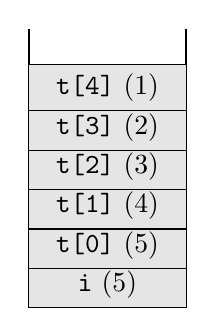
\begin{tikzpicture}
				\tikzstyle{Node} = [rectangle, minimum width=2cm, minimum height=5mm, text centered, draw=black, fill= gray!20]
				\tikzstyle{arrow} = [thick,->,>=stealth]
				
				\draw [thick, black] (0, 0) -- (2, 0);
				\draw [thick, black] (0, 0) -- (0, 3.5);
				\draw [thick, black] (2, 0) -- (2, 3.5);
				\node (c2) [Node] at (1,0.25) {\texttt{i} (5)};
				\node (d2) [Node] at (1,0.75) {\texttt{t[0]} (5)};
				\node (d2) [Node] at (1,1.25) {\texttt{t[1]} (4)};
				\node (d2) [Node] at (1,1.75) {\texttt{t[2]} (3)};
				\node (d2) [Node] at (1,2.25) {\texttt{t[3]} (2)};
				\node (d2) [Node] at (1,2.75) {\texttt{t[4]} (1)};
			\end{tikzpicture}
			\smallskip
			
			A \texttt{main} függvény változói.
		\end{figure}
		\subsection{Biztonsági rések nem definiált viselkedés kihasználásával}
		Irassuk ki a a tömb elemeit! A példa kedvéért rontsuk el a kódot.
		\begin{lstlisting}
for (int i = 0; i < 6; i++) // Hupsz. A csak 5 elem van.
{
	std::cout << t[i] << std::endl;
}
		\end{lstlisting} 
		Itt látható, hogy túl fogunk indexelni. Ez {nem definiált viselkedés}hez vezet. Várhatóan memóriaszemetet fog kiolvasni az utolsó elem helyett, de sose tudhatjuk pontosan mi fog történni. Fordítási időben ezt a hibát a fordító nem veszi észre. A gyakorlaton a programot futtatva nem következett be futási idejű hiba.
		
		Most növeljük meg az elemeket, és indexeljünk túl egészen 100ig!
		\begin{lstlisting}
for (int i = 0; i < 100; i++)
{
	++t[i];
}
std::cout << "sajt" << std::endl;
		\end{lstlisting} 
		Ez a program továbbra is nem definiált viselkedést tartalmaz. Mivel több memóriához nyúlunk hozzá indokolatlanul, ezért nagyobb rá az esély, hogy futási idejű hibába ütközzünk. Az órán a {sajt} szöveg ki lett írva, mégis kaptunk egy szegmentálási hibát (\textit{segmentation fault}).
		
		\begin{lstlisting}
for (int i = 0; i < 100000; i++)
{
	++t[i];
}
std::cout << "sajt" << std::endl;
		\end{lstlisting} 
		A túlindexelést tovább fokozva a program még mielőtt sajt-ot ki tudta volna írni, szegmentálási hibával leállt. Ez jól demonstrálja, hogy ugyanolyan jellegű  a hibát követtük el, de mégis más volt a végeredmény. Ez az egyik ok, amiért veszélyesek a nem definiált viselkedések. Mivel számos különböző hibát okozhatnak, ezért a diagnosztizálásuk sem mindig egyszerű. Az alábbi kód szemléltet egy példát, hogyan lehet biztonsági rés a nem definiált viselkedésből.
		\begin{lstlisting}
#include <iostream>
#include <string>

int main()
{
	int t[] = {5,4,3,2,1};
	int isAdmin = 0;
	std:string name;
	std::cin >> name;
	for (int i = 0; i < name.size(); ++i)
	{
		t[i] = 1;
	}
	if (name == "pityu")
		isAdmin = 1;
	std::cout << "Admin?: " << (isAdmin != 0 ) << std::endl;
}
		\end{lstlisting}
		Ha a programnak \texttt{pityu}-t adunk meg amikor be akarja olvasni \texttt{name}-et, akkor minden rendben. De mivel a forráskódot ismerjük, azért ha hosszú nevet adnánk (nagyobb mint 5), akkor a túlindexelés miatt ki tudjuk használni a nem definiált viselkedéseket. Az is előfordulhat, hogy az \texttt{isAdmin} memóriacímére írunk, és elérjük, hogy a szoftver adminként authentikáljon valakit, aki nem az.
		\medskip
		
		Hogyan lehet ezeket a hibákat elkerülni? Túl azon, hogy figyelni kell, vannak programok amik segítenek. Ehhez használhatunk \texttt{sanitizer}-eket. Ezek módosítanak a fordító által generált kódon. Létrehoz ellenőrzéseket, amik azelőtt észrevesznek bizonyos nem definiált viselkedéseket, mielőtt azok megtörténnének. Pl. itt a túlindexelés, egy futási idejű hibához és egy jól olvasható hibaüzenethez vezetne. Használatukhoz elég egy extra paranccsal fordítanunk:
		
		{\centering\texttt{g++ main.cpp -fsanitize=address}\par }
		
		A sanitizerek csa abban az esetben találnak meg egy hibát, ha a probléma előfordul (azaz futási időben, nem fordítási időben ellenőriz). Amennyiben előfordul, akkor elég pontos leírást tudunk kapni arról, hogy merre van a probléma. Fordítási időben a figyelmeztetések használata segíthet bizonyos hibák elkerülésében.
		
		{\centering \texttt{g++ main.cpp -Wall -Wextra} \par}
		
		A fenti két kapcsoló szintén extra ellenőrzéseket vezet be, de nem változtatják meg a generált kódot.
	\subsection{Hivatkozás tömb elemeire}
		\begin{lstlisting}
#include <iostream>

int main()
{
	int t[] = {5,4,3,2,1};
	int *p = t;
	std::cout << *p << std::endl;
	std::cout << sizeof(int) << std::endl;
	std::cout << sizeof(p) << std::endl;
	std::cout << sizeof(t) << std::endl;
}
		\end{lstlisting}
		Könnyű azt hinni (hibásan), hogy a pointerek ekvivalensek a tömbökkel. A fenti program jól szemlélteti, hogy ez nem igaz. A tömb típusa tartalmazza azt az információt, hogy hány elemű a tömb. Egy pointer típusa csak azt az információt tartalmazza, hogy a mutatott elem mekkora. Számos más különbség is van. A tévhit oka az, hogy tömb könnyen konvertálódik első elemre mutató pointerré.
		
		Egy tömb adott elemére több módon is hivatkozhatunk:
		
		{\centering \texttt{*(p + 3) == *(3 + p) == p[3] == 3[p]} \par}
		\
		\begin{lstlisting}
#include <iostream>

int main()
{
	int t[][3] = {{1,2,3},{4,5,6}};
	return 0;
}
		\end{lstlisting}
		Tekintsük a fenti két dimenziós tömböt. Az első \texttt{[]} jelek közt nincs méret, mert a fordító az inicializáció alapján meg tudja állapítani. A második dimenzió méretének megadása viszont kötelező.
		
		\medskip
		Fentebb a tömböknél megadott ekvivalenciát a mátrixra alkalmazva számos indexelési módot le tudunk vezetni:
		\medskip
		
		\begin{center}
			\texttt{t[1][] == *(*(t+1)+0) == *(1[t]+0) == 0[1[t]] == 0[*(t+1)] == *(t+1)[0] == 1[t][0] } 
		\end{center}
	\begin{note}
		Ahhoz, hogy egy olyan függvényt írjunk, ami minden méretű tömböt elfogad paraméterül, a legegyszerűbb megoldás, ha hagyjuk, hogy a tömb átkonvertálódjon egy első elemre mutató pointerré, és átadjuk külön paraméterben a tömb méretét. Bár van megoldás arra is, hogy egy darab "rugalmas" függvényt írjunk, és az egész tömbről csak egy paramétert vegyünk át. Majd a 7-8. gyakorlaton lesz részletesen szó, de a következő a szintaxis:
		\begin{lstlisting}
template <class T, int ArraySize>
void ( T (&param)[ArraySize] )
{
	//...
}
		\end{lstlisting}
		\smallskip
		A működésének az elvét még nem baj, ha nem értjük. A háttérben egy template paraméter dedukció fog végbemenni: a fordító kitalálja \texttt{param} méretét. 
		
		\smallskip
		A tömbök átvétele paraméterként azért ilyen körülményes, mert egy tömbnek a méretét fordítási időben ismernünk kell. Ha változó méretű tömböt várnánk paraméterül, az szembemenne ezzel a követelménnyel.  
	\end{note}
	\begin{note}
		Előzmény tárgyakból elképzelhető, hogy azt tanultuk, hogy egy tömb méretének egy változót is megadhatunk. Ezt a \texttt{gcc} fordító elfogadja és jó kódot is generál belőle. De ez egy nem szabványos kiterjesztés, ezért nem garantált, hogy ezt minden fordító megteszi. Ez jól demonstrálja, hogy a fordítók nem mindenben követik szorosan a szabványt.
	\end{note}
\end{document}
